\chapter{Results}
\label{chapter:Chapter 5}

This chapter presents what we managed to obtain after implementing \project\ and what how scalable it is.
One of the most important resources is time, and in \labelindexref{Figure}{img:time-for-starting-vms} we present how using \project\ scales when starting up the VMs.
The image shows on the horizontal axis the number of VMs that were started for a given run and on the vertical axis the time it took from when the user submitted the \texttt{start_all} command until every machine has booted.
There were 10 runs for each data point, and we plotted the average, minimum and maximum runs to ensure that the results are not biased by the system load at the time the benchmark was run.
We can see that the deviation from the average is not very big, concluding that the test results are stable.

\begin{figure}[htb]
	\begin{center}
	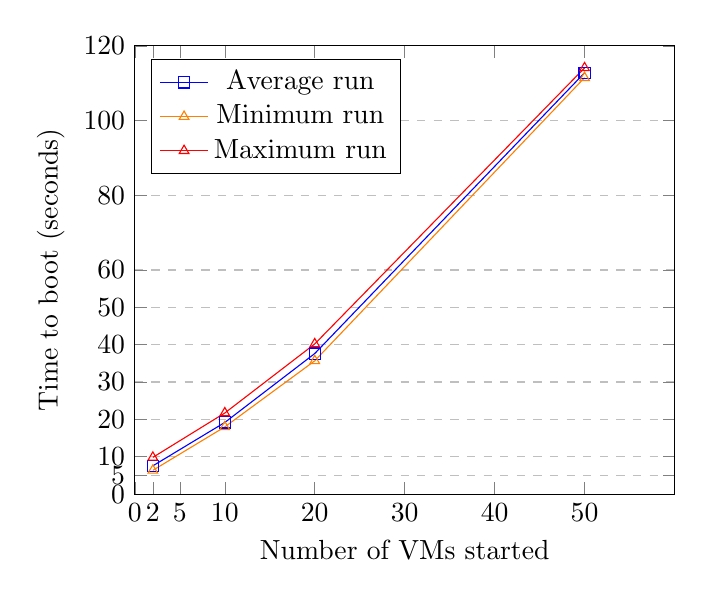
\begin{tikzpicture}
	\begin{axis}[
		xlabel={Number of VMs started},
		ylabel={Time to boot (seconds)},
		xmin=0, xmax=60,
		ymin=0, ymax=120,
		xtick={0,2,5,10,20,30,40,50},
		ytick={0,5,10,20,30,40,50,60,80,100,120},
		legend pos=north west,
		ymajorgrids=true,
		grid style=dashed,
	]

	\addplot[
		color=blue,
		mark=square,
		]
		coordinates {
		(2,7.5708)(10,19.1846)(20,37.6299)(50,112.773)
		};
		\legend{Average run}

	\addplot[
		color=orange,
		mark=triangle,
		]
		coordinates {
		(2,6.368)(10,17.991)(20,35.679)(50,111.464)
		};
		\addlegendentry{Minimum run}

	\addplot[
		color=red,
		mark=triangle,
		]
		coordinates {
		(2,9.84)(10,21.716)(20,40.201)(50,114.082)
		};
		\addlegendentry{Maximum run}

	\end{axis}
	\end{tikzpicture}
	\caption{Scalability of starting the VMs \label{img:time-for-starting-vms}}
	\end{center}
\end{figure}

The benchmark was run on a system with 12GB of RAM, a quad core processor clocked at 2.6GHz, running an operating system based with Linux Kernel 3.14.
For the general case, a user would not need more than 20 \texttt{Hosts} within his topology to test a protocol, but for reference we tested for 50 \texttt{Hosts} as well.

Without \project, one would need to manually create, start and configure VMs created with Virtual Box or VMWare, a process which would take a lot more than 1-2 minutes.
Also, another important aspect that we realized with \project\ is the fact that because we used a shared folder that is used by every VM, we actually saved a lot of disk space.
Before, one would need a lot more space because every VirtualBox or VMWare VM needed its own disk, duplicating much data.
For example, we only need around 50MB of disk space for the Linux Image and the other tools like Dropbear and BusyBox.
This is valid even if we start one machine or 100.
With the old solutions, the space used was growing linearly with the number of machines, like for one machine we would need let's say 700MB of disk space, but when we scale that to 20 machines, it means over 13GB of disk space, just for the machines.

In terms of RAM usage, things have also improved, because we can give the VMs exactly as much RAM as the Linux Kernel needs to run, which could be as low as 64MB of RAM.
By using the other solutions, we would need to run the operating systems themselves, which would require more than 192MB of RAM for each machine.
In terms of scaling, this means that we could use over 100 VMs on our machine with \project\ without any problems, while other solutions we would be capped at only 30-40 machines.
